\documentclass{article}

\usepackage{graphicx}
\usepackage{hyperref}
\usepackage{listings}
\usepackage{color}
\usepackage{verbatim}
\usepackage{amsmath}
%\usepackage{subfig}
\usepackage{caption}
\usepackage{subcaption}



\begin{document}
\section{Methodology}
\subsection{Graph Partitioning}
In studying 'small world' networks proposed by Watts and Strogatz \cite{Watts:1998} Fan Chung and Linyuan Lu propose an algorithm that separates a graph into a locally connected component and a teleportation component. This essentially breaks a graph into a group of edges between highly connected nodes with many paths between them, and the remainder of the edges between far sparsely connected nodes. Given integers $k \geq 2$ and $l \geq 2$, a $(k,l)$ locally connected graph will have at least $l$ paths connecting any given two nodes with distinct edges in each path. The length of each path can be at most $k$ edges for this pair. A grid network can be described locally with $k=3$ and $l=3$, and is a good example of how a planar graph is connected. I set these values for $k$ and $l$ for the remainder of the paper. Given graph, $G$, its maximum $k,l$-locally connected subgraph is the union of all $k,l$-locally connected subgraphs within the entire graph. It is important that this maximum is unique, and can be found through an iterative edge deletion algorithm \cite{Chung:2004}. Search through all edges in the graph, and remove an edge if it does not have at least $l$ edge-disjoint paths of length less than or equal to $k$. Repeat this cycle until no edges can be removed. Chung and Lu prove that this algorithm succeeds regardless of the order of edges removed \cite{Chung:2004}. 

\subsubsection{Partitioning Algorithm}
Graph G\\
P = copy(G)\\
While: $Deleted\_edges == True$:\\
\indent Deleted\_edges = False\\
\indent For $edge$ in P.edges:\\
\indent \indent $(start\_node, end\_node) = edge$\\
\indent \indent Search through paths of length $i=2:k$ from $start\_node$ to $end\_node$\\
\indent \indent $count =$  number of edge-disjoint paths\\
\indent \indent if $count \leq l$:\\
\indent \indent \indent P.remove($edge$)\\
\indent \indent \indent $Deleted\_edges = $True\\
$P$ is the maximum $k,l$-locally connected subgraph of G.
	


\begin{figure}
\centering
\begin{subfigure}{.5\textwidth}
  \centering
  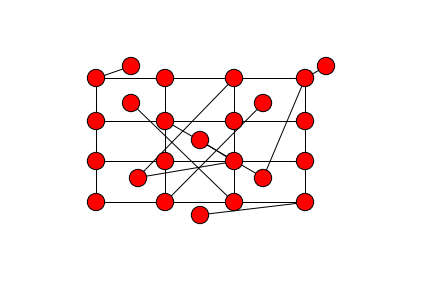
\includegraphics[width=\linewidth]{entiregraph.png}
  \caption{G, grid with random edges}
  \label{fig:sub1}
\end{subfigure}%
\begin{subfigure}{.5\textwidth}
  \centering
  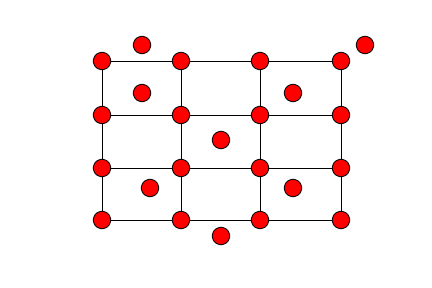
\includegraphics[width=\linewidth]{planargraph.png}
  \caption{P, max (3,3)-l. c. subgraph of G}
  \label{fig:sub2}
\end{subfigure}
\caption{Partitioning algorithm results in planar locally connected subgraph}
\label{fig:test}
\end{figure}

\subsubsection{NetworkX Library and My Additions}
There is an open source Python library for graph theory and computation called NetworkX written by Hagberg, Schult, and Swart from Los Alamos National Lab. I use many of their functions for reading through edgelists, computing node degrees, converting graphs to Laplacian matrices, etc which are incredibly useful for simple graph work \cite{Hagberg:2008}. Included in this package is a function for finding the locally connected subgraph of a graph based upon the work of Chung-Lu above (cite?). Throughout much of the course of my work I used this function to partition my graphs. However for graphs with many edges, this function adds a huge time complexity overhead because it utilizes a shortest path algorithm (cite Dijkstra?) to test each edge's connectivity. This algorithm has similar complexity for any given $k$, $l$ connected subgraphs, however I only care about $k,l = 3$. Thus I wrote an optimized code that simply searches through all potential paths of length 2 and 3 in the graph. This requires much less work than running a shortest path algorithm several thousand times. In the process, and after much debugging and testing, I think that the established NetworkX function has some errors. I now only use my simplified code which speeds up the overall algorithm greatly. Results for partitioning timing are included in the Results section. I hope to work more on my code and submit it as an open-source contribution to the NetworkX package. The established function for partitioning a graph is still important, however, and I hope to work further to find the errors in the function.

\subsection{Laplacian Solver}
I have partitioned a graph into its locally connected subgraph, $P$, and the graph of the teleportation edges, $T$. These subgraphs can be converted to Laplacian form with $P_L$ matrix of connections and degree information for the locally connected part, and $T_L$, similar for the teleportation part. With a minor diagonal operation on $T_L$, we have $L = P_L + T_L$ where $L$ is the Laplacian for the entire graph. To solve a Laplacian linear system $Lx=b$ we now solve the two subgraph Laplacians and use linear algebra.

\subsubsection{Linear Algebra: Woodbury Matrix Identity}
I utilize the Woodbury matrix Identity:\\
\begin{center}
$(A+UCV)^{-1} = A^{-1} - A^{-1}U(C^{-1}+VA^{-1}U)^{-1}VA^{-1}$\\
\end{center}
with A replaced by $P_L$, $U$ and $V$ component matrices of the SVD of $T_L$, and $C$ replaced by a diagonal of the singular values of $T_L$. For a class of graphs we will assume that $P_L$ is very large and sparse, and $T_L$ is very sparse and low rank. Here is a breakdown of how I solve the Laplacian linear system:

\begin{align*}
Lx & = b\\
x & = L^{-1}b\\
x & = (P_L+T_L)^{-1}b\\
x & = (P_L+USV)^{-1}b\\
x & = (P_L^{-1}-P_L^{-1}U(S^{-1}+VP_L^{-1}U)^{-1}VP_L^{-1})b\\
x & = P_L^{-1}b-P_L^{-1}U(S^{-1}+VP_L^{-1}U)^{-1}VP_L^{-1}b\\
\end{align*}


\subsubsection{Algebraic Multigrid of Locally Connected Subgraph}
The locally connected subgraph is planar, meaning it can be drawn on a piece of paper without any edges crossing (proof it is planar?). Using work beginning with Gary Miller \cite{Miller:1995}, we know that an Algebraic Multigrid solver is optimal for this planar graph laplacian matrix as the solution space is split into multiple cycles of coarsened solving \cite{Brandt:1984}. Previous approaches to using multigrid (LAMG, CMG, Cascadic) to solve Laplacian linear systems do not have a systematic method of graph coarsening. They are based on heuristics for identifying which edges to keep in the multiple levels. Whereas these algorithms are prone to losing edge information in the multiple coarsening cycles, my algorithm runs multigrid only on the planar portion, preserving correct edge information in the coarse levels. (do i need to cite?)There are many multigrid solves in this algorithm, and it is important to optimize performance. Thus I use the Portable, Extensible Toolkit for Scientific Computation (PETSc) and its python library petsc4py to run multigrid solves \cite{petsc-user-ref, Dalcin:2011}

\subsubsection{Low Rank SVD of Teleportation Subgraph}
The Woodbury matrix identity requires use of the singular value decomposition for the teleportation laplacian $T_L$. For graphs I am interested in, the number of edges in the Teleportation subgraph is very small relative to the size of the original graph. This causes the laplacian matrix of teleportation subgraph, $T_L$, to have very low rank structure. Currently I am taking the full-rank SVD of $T_L$ and removing the columns of U and rows of V that correspond to negligible singular values. Given $n\times n$ matrix $T_L$ with rank $r$, we compute $USV = T_L$ where $T_L$ has $r$ non-negligible singular values. Thus U is tall-skinny $n\times r$, S is an $r\times r$ diagonal matrix of the non-negligible singular values, and V is short-fat $r\times n$. The full rank SVD has $O(n^3)$ complexity and dominates the complexity of the entire method. However, in future work I can take the low rank singular value decomposition (cite?) to solve this small portion which has $O(r^2 n)$ complexity. This change will be very valuable in solving many-node networks.

\subsection{Model Complexity}
\subsubsection{Graph Splitting}
The small-world networks that Watts-Strogatz and Chung-Lu worked with roughly follow a power law degree distribution where the proportion of nodes with $d$ degree scales with $d^{-\gamma}$ with $2 < \gamma < 3$ \cite{Chung:2004,Watts:1998}. In lay terms, there are a few nodes with high degree and many nodes with low degree ($\leq3$ e.g.). This is similar to an exponential distribution, however a power law distribution has a much longer and fatter tail. Given probability density function of the degree distribution: $P(d)$, we can compute the expected degree in a sequence $E[d]$ with $\zeta(x)$, the Riemann-zeta function:\\
\begin{align*}
P(d) & = \frac{d^{-\gamma}}{\zeta(\gamma)},               \zeta(s) = \sum_{n=1}^{\infty} \frac{1}{n^s}\\
E[d] & = \sum_{d=1}^{\infty} d \frac{d^{-\gamma}}{\zeta(\gamma)} \\
E[d] & = \frac{\zeta(\gamma-1)}{\zeta(\gamma)}\\ 
\end{align*}
As $\gamma$ increases from two to three, the expected value of the distribution decreases. For most realistic values of $\gamma$, the expected value is small, and this is why they are sometimes described as graphs with "preferential attachment"; edges are added between nodes that already have many edges. It is important to note that graphs with finite nodes can be described with $\gamma \leq 2$. The degree decay of these distributions is stretched. These stretched power law distributions do not have an expected value because they are not well-defined for node numberings approaching infinity, however an average value can be calculated over a set of finite nodes. This might be a more appropriate fit for datasets described in the Results section.\\
\begin{figure}
\begin{center}
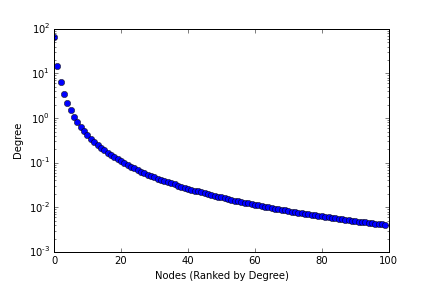
\includegraphics[width=\linewidth]{powerlawdeg.png}
  \caption{Degree sequence of power-law distribution, $\gamma = 2.1$\\
  Note the rapid degree decay after the first 5 nodes.}
  \end{center}
  \end{figure}

For now, let's assume our degree sequence follows the original power law distribution. To partition the graph using Chung-Lu for $k = 3$ and $l = 3$, for each node we must search through all paths of lengths 1, 2, and 3 away from the node. We only continue if path of length 1 exists. If so, we take the expected value of the degree sequence and raise it to the second power to give number of paths of length 2. We do it similarly for the third power. This gives us expected number of paths: $(E[d])^{2}+(E[d])^{3}$. Then it is simple to count the number of edge-disjoint paths. If there are two or less edge-disjoint paths, the edge (path length 1) is removed. For a graph with m edges, this requires $m*((E[d])^{3})$ searches for one iteration of the cycle. For computational complexity of real-world graphs, simply replace the $E[d]$ value with the calculated average degree. We continue iterating this cycle until no edges can be removed. I do not have a bound on the number of iterations required to remove all teleportation edges, however in experiments with real-world graphs, it seems they require two iterations at most (see results).

\subsubsection{Linear Algebra and Solves}
After splitting the entire graph into locally-connected subgraph and teleportation subgraph, we must count the number of floating point operations (FLOPs) for each operation in the method. Listed are the operations with flop count for $n\times n$ matrices $P_L$ and rank-r $T_L$, $n\times r$ matrix U, $r\times r$ matrix S, $r\times n$ matrix V, and $n\times 1$ vector, b:\\
\begin{center}
\renewcommand{\arraystretch}{1.5}
    \begin{tabular}{ | l | l |}
    \hline
    \textbf{Operation} & \textbf{O(FLOPs)} \\ \hline
    $USV = T_L$ & $O(n^3)$ \\ \hline
    $S^{-1}$ & $O(r)$ \\ \hline
    $y = P_L^{-1}b$ (MG) & O(n)  \\  \hline
    $y_1 = Vy$ & $O(rn)$ \\ \hline
    $Q = P_L^{-1}U$ ($r$ MG solves) & $O(rn)$ \\ \hline
    $Q_1 = VQ$ & $O(r^2 n)$ \\ \hline
    $Q_2 = S^{-1} + Q_1$ & $O(r^2)$ \\ \hline
    $y_2 = Q_2^{-1}y_1$ & $O(r^3)$ \\ \hline
    $y_3 = Uy_2$ & $O(rn)$ \\ \hline
    $y_4 = P_L^{-1}y_3$ (MG) & $O(n)$ \\ \hline
    $x = y - y_4$ & $O(n)$ \\
    \hline
    \end{tabular}
\end{center}
In summary: given $n\times n$ graph Laplacian matrix and rank-r teleportation matrix, the method is $O(n^3)$, however with work to implement the low rank SVD, it is $O(r^3+r^2 n)$. It is clear that the complexity of the solve depend on $r$, the rank of the teleportation matrix $T_L$. We will show in the results section how the theoretical complexity of the algorithm compares to the calculated timings for the graph partitioning and each operation in the linear system solve.





%\bibliographystyle{siam}
%\bibliography{mastersbib}


\end{document}